\chapter{Substrate-free sample delivery}
In FXI everything that is illuminated by the X-ray pulse is sample. In the case of weakly scattering single particles scattering from any substrate around the might drown the signal from the particle itself. Aerosol injection removes this clutter and assures that the sample is clearly isolated from its surroundings, and this, as we see in a later chapter 6, is important for image recovery.

An aerosol injector produces small droplets of particles dissolved in a volatile buffer. The buffer evaporates under the reduced pressure inside the experimental chamber, ideally leaving behind only the particle. There are two main types of nozzles that can be used to produce small drops: the Gas Dynamic Virtual Nozzle, and electro spray ionisation (ESI).

\begin{figure}[h]\label{fig:drop_formation}
\centering 
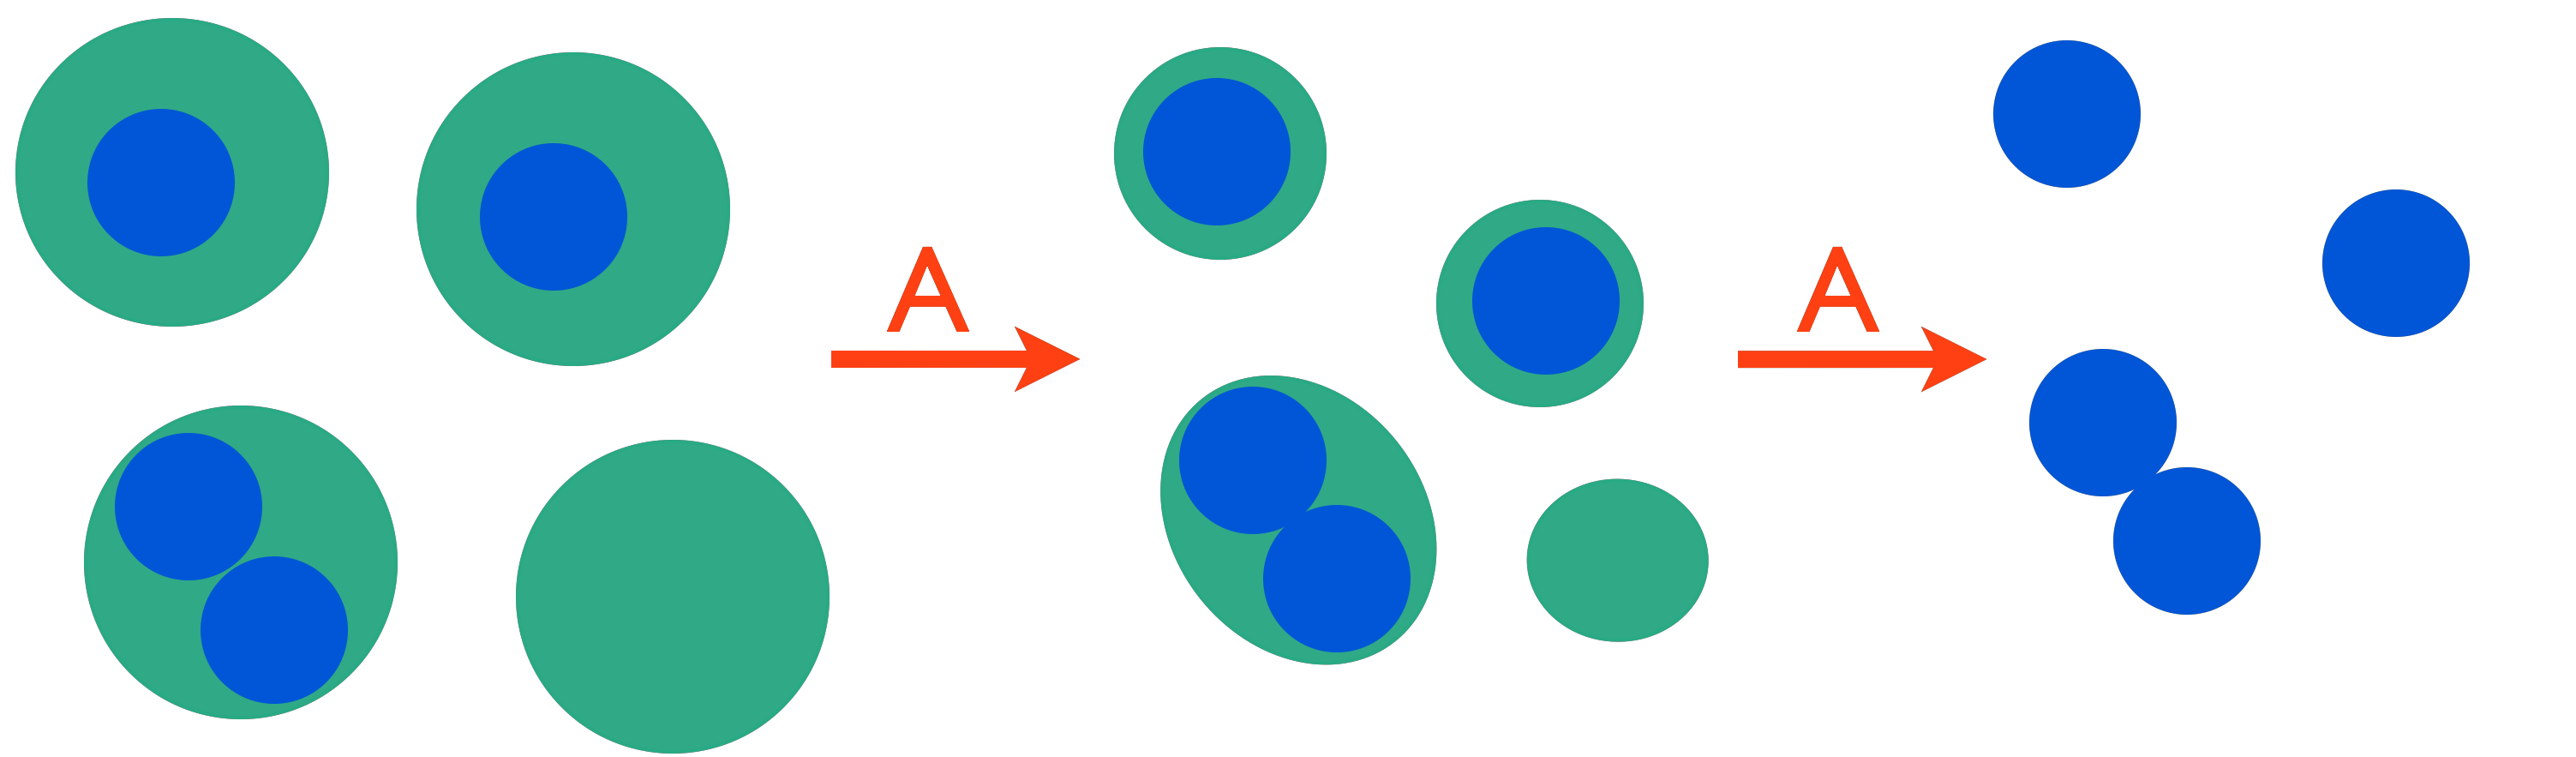
\includegraphics[width=120mm]{Chapter_04_GDVNEvaporation.png}
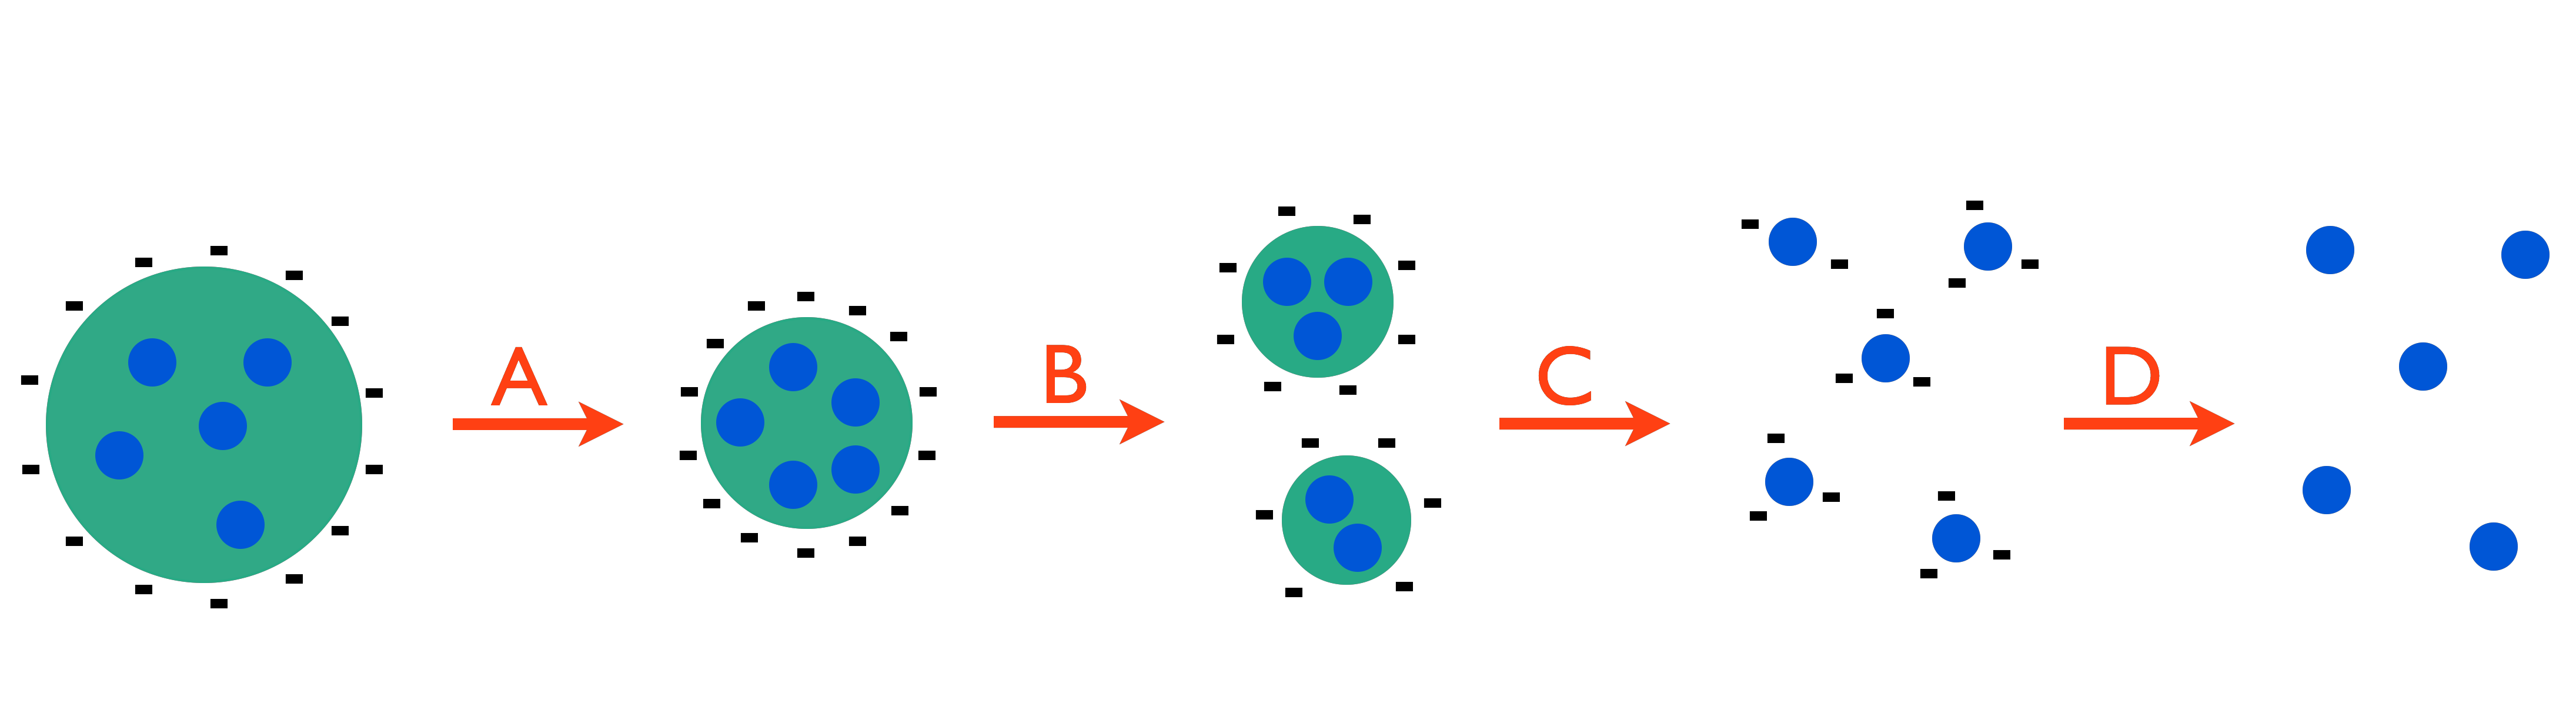
\includegraphics[width=120mm]{ESI_drop_evaporation_explosion.png}

\caption{Experimental geometry, including different sample delivery system. From the bottom left the x-rays pulses enter the chamber. The experimentalist can now select a sample delivery system. Shown are an aerosol sample delivery system, liquid jet injection system, and two types of substrate bound sample delivery systems. If the beam intersect the sample (and/or substrate) a diffraction pattern is recorded on two sets of detectors, placed at different distances from the interaction region.}
\end{figure}




\subsection{Gas Dynamic Virtual Nozzle}

If the coaxial flow of gas creates a jet with a diameter smaller than then a characteristic $d_j$ the surface tension in the liquid will cause the jet to break up into a mist of small droplets. $d_j$ can be estimated on the basis of energy conservation, and is a function of the effective pressure drop $\Delta P$. It is assumed that all energy is transformed to kinetic energy \cite{Acero2013}.
\begin{equation}
d_j^{(GDVN)} = 2 \sqrt{Q \cdot \left(\frac{\rho}{2 \pi^2 \Delta P}\right)^{1/2}}
\end{equation}    
$Q$ denotes the flow rate and $\rho$ is the density of the liquid. The final drop diameter $d_d$ can be related to the jet diameter using the ratio $d_d / d_j \approx 1.9$, which is the classical Rayleigh breakup []. Empirically this assumption has been shown to work well for low-viscosity media such as water. The GDVN can create droplets in the size range of 400 nm - 2000 nm. Sample consumption is in the range of ul/min.

\subsection{Aerodynamic Lens Stack}
After the droplets formed, they start to evaporate in the reduced pressure environment, leaving only the non-volatile particles in the 'drop'. The aerosolised particles are guided into an aerodynamic lens stack (see figure ). This is a series of cylindrical cavities, connected by co-aligned orifices, that collimate the droplets into a narrow beam of particles [].

\begin{figure}[h]\label{fig:skimmer_aerolens}
\centering 
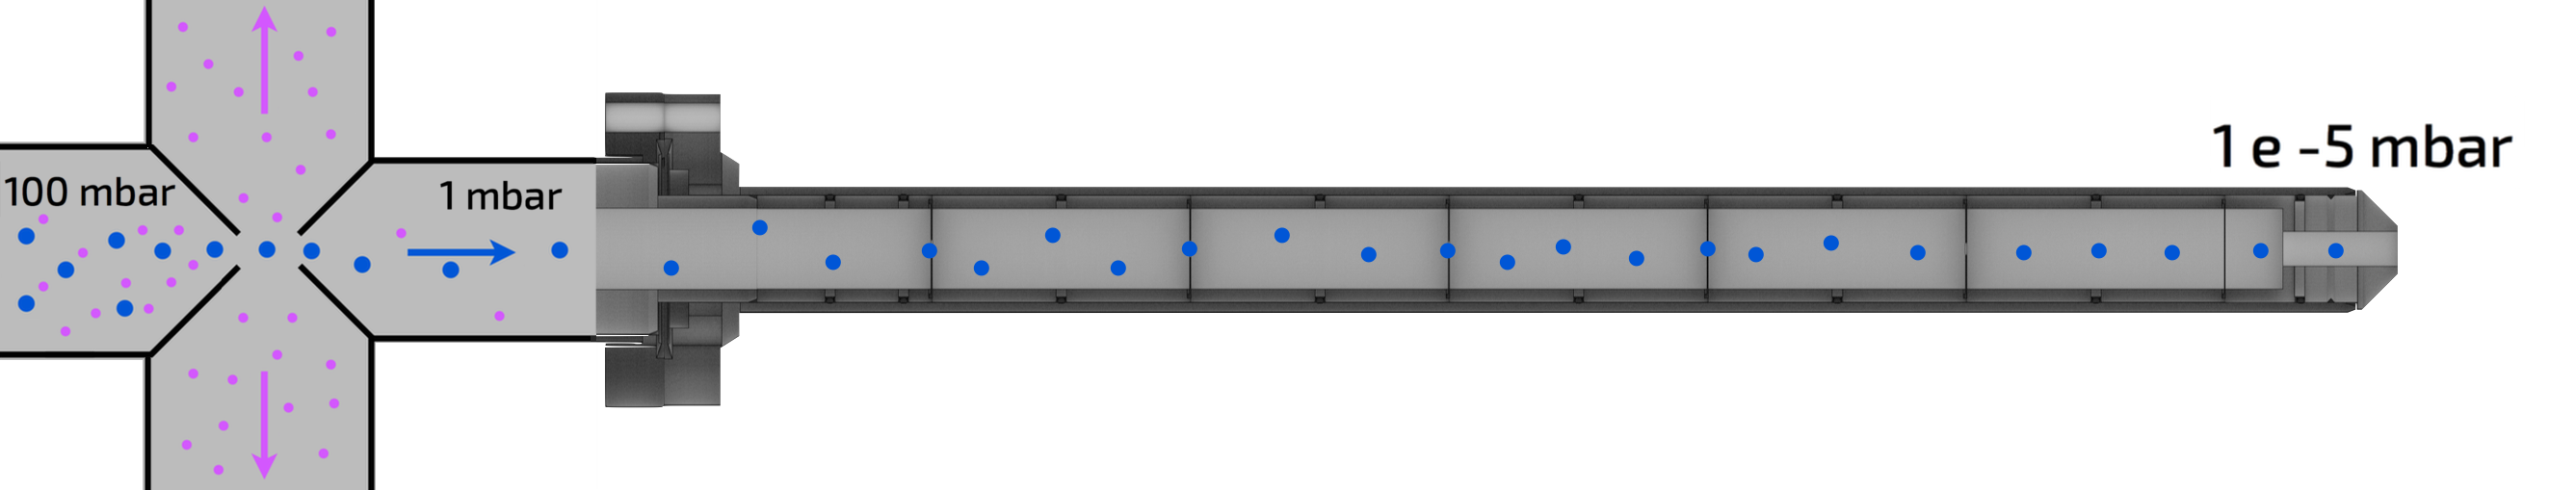
\includegraphics[width=120mm]{Chapter_04_SkimmerAerodynamicLens.png}
\caption{Experimental geometry, including different sample delivery system. From the bottom left the x-rays pulses enter the chamber. The experimentalist can now select a sample delivery system. Shown are an aerosol sample delivery system, liquid jet injection system, and two types of substrate bound sample delivery systems. If the beam intersect the sample (and/or substrate) a diffraction pattern is recorded on two sets of detectors, placed at different distances from the interaction region.}
\end{figure}

For robust particles, which are large compared to the drop size, this type of sample injection has proven to be very successful. This sample injection method made it possible to measure the diffraction patterns from isolated single particles at high signal-to-noise ratios at very high repetition rates. Up to 80\% hit rates have been recorded with a 120 Hz repetition rates at the LCLS \cite{Hantke2013}. The results discussed in this thesis come from datasets that were generated using the GVDN injection method.

For many samples aerosol injection is not disruptive. Molecular dynamics simulation have shown that the conformation of proteins is conserved up till the moment that the last structural water evaporates[]. For the cyanobacterial cells described in this paper it has been shown that the shape and the autofluorescence properties of the cell membranes of the injected cells remain unchanged [PAPER I]. This is not quite unexpected. Aerosols of cyanobacteria can be carried for long distances, and metabolically active cells have been detected at altitudes of 20-70 km where atmospheric pressure drops to below a millibar []. Other sample cell lines such as \textit{E. coli} and brewers yeast, and many types of viruses have been shown to be viable after injection. Nevertheless, not all sample types may be amenable to aerosol sample injection, and samples should be tested prior to experiments.  

\subsection{Electro Spray Ionisation}
Over the last years it became apparent that GDVN sample injection does have its limitations. If the particle becomes small compared to the drop size, wide size distributions of otherwise uniformly sized particles were measured [Daurer, Hantke]. These observations might be explained by a combination of an incomplete evaporation process, and the build up of a significant shell of debris, originating from impurities present in the solution, around the particle. To purify the measured sample, smaller drops had to be generated. A common aerosolisation technique used in mass spectrometry called electro spray ionisation (ESI) is known to be able to produce small droplets.

ESI nozzles produce droplets through a similar droplet formation process as occurs in the GDVN. The difference lies in the process that drives jet acceleration. In ESI the jet is accelerated by an externally applied electrostatic potential. In the capillary the solvent (volatile buffer) is mixed with negatively charged ions. By applying an external field these ions are accelerated, accelerating the entire jet. The accelerated jet will ultimately break into small drops similar to what occurs in a GDVN. The characteristic $d_j^{ESI}$ can be described as a function of the surface tension $\sigma$, vacuum permittivity $\varepsilon_0$, electrical conductivity $C$, as well as the flow rate and the density of the liquid.
\begin{equation}
d_j^{(ESI)} \approx 2 \sqrt{Q \cdot \left(\frac{\rho \varepsilon_0}{\sigma C}\right)^{1/3}}
\end{equation}

After the process of evaporation initiates, an electric potential further builds up in the drops, eventually leading to a Coulomb explosion of the drops [Cole]. Cycles of evarporation and explosion leads to smaller and smaller drops. Initial experiments showed that drops of mono disperse droplets of size 150-200 nm can be generated with ESI. ESI can also be combined with an aerodynamic lens stack. 

The transfer of ESI to FXI is a considerable achievement that will allow the field to move forward to image smaller particles such as proteins. This would not have been possible using the GDVN aerosolisation. ESI has been shown to also function under lower flowrates, reducing sample consumption to 10 nl/min []. This sample consumption rate is advantageous for samples that are only available in small quantities. 

\subsection{Drop-on-demand}
The combination of ESI and a quadrupole with an ion trap for storage allows for a pulsed delivery system that can be tuned to match the repetition rate of the XFEL. This is generally referred to as drop-on-demand. This would reduce the sample consumption even further. Moreover the ion trap can also be utilized for sample selection prior to injection of sample into the x-ray pulse. This is important for single proteins as they scatter very little signal, which makes it very difficult to separate the diffraction patterns from the particle-of-interest and those diffraction patterns obtained from contaminating particles or other noise. 

